%        File: nuc_models.tex
%     Created: Wed Oct 09 02:00 PM 2013 P
% Last Change: Wed Oct 09 02:00 PM 2013 P
%

%
% Copyright 2007, 2008, 2009 Elsevier Ltd
%
% This file is part of the 'Elsarticle Bundle'.
% ---------------------------------------------
%
% It may be distributed under the conditions of the LaTeX Project Public
% License, either version 1.2 of this license or (at your option) any
% later version.  The latest version of this license is in
%    http://www.latex-project.org/lppl.txt
% and version 1.2 or later is part of all distributions of LaTeX
% version 1999/12/01 or later.
%
% The list of all files belonging to the 'Elsarticle Bundle' is
% given in the file `manifest.txt'.
%

% Template article for Elsevier's document class `elsarticle'
% with numbered style bibliographic references
% SP 2008/03/01
%
%
%
% $Id: elsarticle-template-num.tex 4 2009-10-24 08:22:58Z rishi $
%
%
\documentclass[preprint,12pt]{elsarticle}

% Use the option review to obtain double line spacing
% \documentclass[preprint,review,12pt]{elsarticle}

% Use the options 1p,twocolumn; 3p; 3p,twocolumn; 5p; or 5p,twocolumn
% for a journal layout:
% \documentclass[final,1p,times]{elsarticle}
% \documentclass[final,1p,times,twocolumn]{elsarticle}
% \documentclass[final,3p,times]{elsarticle}
% \documentclass[final,3p,times,twocolumn]{elsarticle}
% \documentclass[final,5p,times]{elsarticle}
% \documentclass[final,5p,times,twocolumn]{elsarticle}

% if you use PostScript figures in your article
% use the graphics package for simple commands
% \usepackage{graphics}
% or use the graphicx package for more complicated commands
\usepackage{graphicx}
% or use the epsfig package if you prefer to use the old commands
% \usepackage{epsfig}

% The amssymb package provides various useful mathematical symbols
\usepackage{amssymb}
% The amsthm package provides extended theorem environments
% \usepackage{amsthm}
\usepackage{amsmath}

% The lineno packages adds line numbers. Start line numbering with
% \begin{linenumbers}, end it with \end{linenumbers}. Or switch it on
% for the whole article with \linenumbers after \end{frontmatter}.
\usepackage{lineno}

% I like to be in control
\usepackage{placeins}

% The glossaries package gives me acronym expansion
\usepackage[acronym,toc]{glossaries}
\newacronym{MIT}{MIT}{the Massachusetts Institute of Technology}
\newacronym{UW}{UW}{University of Wisconsin}
\newacronym{US}{US}{United States}
\newacronym{IAEA}{IAEA}{International Atomic Energy Agency}
\newacronym{SNF}{SNF}{spent nuclear fuel}
\newacronym{HLW}{HLW}{high level waste}
\newacronym{FEHM}{FEHM}{Finite Element Heat and Mass Transfer}
\newacronym{DOE}{DOE}{Department of Energy}
\newacronym{GENIUSv1}{GENIUS}{Global Evaluation of Nuclear Infrastructure
Utilization Scenarios, Version 1}
\newacronym{GENIUSv2}{GENIUS}{Global Evaluation of Nuclear Infrastructure Utilization Scenarios, Version 2}
\newacronym{CNERG}{CNERG}{Computational Nuclear Engineering Research Group}
\newacronym{GDSM}{GDSM}{Generic Disposal System Model}
\newacronym{GDSE}{GDSE}{Generic Disposal System Environment}
\newacronym{GPAM}{GPAM}{Generic Performance Assessment Model}
\newacronym{FEPs}{FEPs}{Features, Events, and Processes}
\newacronym{EBS}{EBS}{Engineered Barrier System}
\newacronym{EDZ}{EDZ}{Excavation Disturbed Zone}
\newacronym{YMR}{YMR}{Yucca Mountain Repository Site}
\newacronym{EPA}{EPA}{Environmental Protection Agency}
\newacronym{PEI}{PEI}{Peak Environmental Impact}
\newacronym{VISION}{VISION}{the Verifiable Fuel Cycle Simulation Model}
\newacronym{NUWASTE}{NUWASTE}{Nuclear Waste Assessment System for Technical Evaluation}
\newacronym{NWTRB}{NWTRB}{Nuclear Waste Technical Review Board}
\newacronym{OCRWM}{OCRWM}{Office of Civilian Radioactive Waste Management}
\newacronym{UFD}{UFD}{Used Fuel Disposition}
\newacronym{DYMOND}{DYMOND}{Dynamic Model of Nuclear Development }
\newacronym{DANESS}{DANESS}{Dynamic Analysis of Nuclear Energy System Strategies}
\newacronym{CAFCA}{CAFCA}{ Code for Advanced Fuel Cycles Assessment }
\newacronym{ORION}{ORION}{O..}
\newacronym{NFCSim}{NFCSim}{Nuclear Fuel Cycle Simulator}
\newacronym{COSI}{COSI}{Commelini-Sicard}
\newacronym{FCT}{FCT}{Fuel Cycle Technology}
\newacronym{SWF}{SWF}{Separations and Waste Forms}
\newacronym{FCO}{FCO}{Fuel Cycle Options}
\newacronym{RDD}{RD\&D}{Research Development and Design}
\newacronym{WIPP}{WIPP}{Waste Isolation Pilot Plant}
\newacronym{ANDRA}{ANDRA}{Agence Nationale pour la gestion des D\'echets RAdioactifs, the French National Agency for Radioactive Waste Management}
\newacronym{TSM}{TSM}{Total System Model}
\newacronym{LANL}{LANL}{Los Alamos National Laboratory}
\newacronym{INL}{INL}{Idaho National Laboratory}
\newacronym{ANL}{ANL}{Argonne National Laboratory}
\newacronym{SNL}{SNL}{Sandia National Laboratory}
\newacronym{LBNL}{LBNL}{Lawrence Berkeley National Laboratory}
\newacronym{LLNL}{LLNL}{Lawrence Livermore National Laboratory}
\newacronym{NAGRA}{NAGRA}{National Cooperative for the Disposal of Radioactive Waste}
\newacronym{CUBIT}{CUBIT}{CUBIT Geometry and Mesh Generation Toolkit}
\newacronym{CSNF}{CSNF}{Commercial Spent Nuclear Fuel}
\newacronym{DSNF}{DSNF}{DOE Spent Nuclear Fuel}
\newacronym{MTHM}{MTHM}{Metric Ton of Heavy Metal}
\newacronym{HTGR}{HTGR}{High Temperature Gas Reactor}
\newacronym{TRISO}{TRISO}{Tristructural Isotropic}
\newacronym{MA}{MA}{Minor Actinide}
\newacronym{CEA}{CEA}{Commissariat a l'Energie Atomique et aux Energies Alternatives}
\newacronym{SKB}{SKB}{Svensk Karnbranslehantering AB}
\newacronym{SINDAG}{SINDA{\textbackslash}G}{Systems Improved Numerical Differencing Analyzer $\backslash$ Gaski}
\newacronym{STC}{STC}{Specific Temperature Change}
\newacronym{LDRD}{LDRD}{Laboratory Directed Research and Development}
\newacronym{LCOE}{LCOE}{Levelized Cost of Electricity}
\newacronym{ABM}{ABM}{Agent-Based Modeling}
\newacronym{COTS}{COTS}{Commercial, Off-The-Shelf}
\newacronym{API}{API}{Application Programming Interface}
\newacronym{RIF}{RIF}{Region-Institution-Facility}
\newacronym{GUI}{GUI}{Graphical User Interface}
\newacronym{HPC}{HPC}{High-Performance Computing}
\newacronym{HTC}{HTC}{High-Throughput Computing}
\newacronym{UML}{UML}{Unified Modeling Language}
\newacronym{DAG}{DAG}{Directed Acyclic Graph}
\newacronym{MOX}{MOX}{Mixed Oxide}
\newacronym{UOX}{UOX}{Uranium Oxide}
\newacronym{QA}{QA}{Quality Assurance}
\newacronym{NQA1}{NQA-1}{Nuclear Quality Assurance - 1}
\newacronym{VV}{V\&V}{Verification and Validation}
\newacronym{UQ}{UQ}{Uncertainty Quantification}
\newacronym{ASME}{ASME}{American Society of Mechanical Engineers}
\newacronym{NEAMS}{NEAMS}{Nuclear Engineering Advanced Modeling and Simulation}
\newacronym{CI}{CI}{Continuous Integration}
\newacronym{DRE}{DRE}{Dynamic Resource Exchange}
%\newacronym{<++>}{<++>}{<++>}

\makeglossaries

% natbib.sty is loaded by default. However, natbib options can be
% provided with \biboptions{...} command. Following options are
% valid:

%   round  -  round parentheses are used (default)
%   square -  square brackets are used   [option]
%   curly  -  curly braces are used      {option}
%   angle  -  angle brackets are used    <option>
%   semicolon  -  multiple citations separated by semi-colon
%   colon  - same as semicolon, an earlier confusion
%   comma  -  separated by comma
%   numbers-  selects numerical citations
%   super  -  numerical citations as superscripts
%   sort   -  sorts multiple citations according to order in ref. list
%   sort&compress   -  like sort, but also compresses numerical citations
%   compress - compresses without sorting
%
% \biboptions{comma,round}

% \biboptions{}


% Katy Huff addtions
\usepackage{xspace}
\newcommand{\Cyclus}{\textsc{Cyclus}\xspace}%
\newcommand{\Cyder}{\textsc{Cyder}\xspace}%
\usepackage{color}
\DeclareMathOperator{\erf}{erf}
\DeclareMathOperator{\erfc}{erfc}


 \journal{Progress in Nuclear Energy}

\begin{document}

\begin{frontmatter}

   % Title, authors and addresses

   % use the tnoteref command within \title for footnotes;
   % use the tnotetext command for the associated footnote;
   % use the fnref command within \author or \address for footnotes;
   % use the fntext command for the associated footnote;
   % use the corref command within \author for corresponding author footnotes;
   % use the cortext command for the associated footnote;
   % use the ead command for the email address,
   % and the form \ead[url] for the home page:
   %
   % \title{Title\tnoteref{label1}}
   % \tnotetext[label1]{}
   % \author{Name\corref{cor1}\fnref{label2}}
   % \ead{email address}
   % \ead[url]{home page}
   % \fntext[label2]{}
   % \cortext[cor1]{}
   % \address{Address\fnref{label3}}
   % \fntext[label3]{}

\title{Rapid Methods for Radionuclide Contaminant Transport in Nuclear Fuel Cycle Simulation}

   % use optional labels to link authors explicitly to addresses:
   % \author[label1,label2]{<author name>}
   % \address[label1]{<address>}
   % \address[label2]{<address>}

\author[berk]{Kathryn Huff}
  \ead{huff@berkeley.edu}
  \address[berk]{Department of Nuclear Engineering, University of California, 2521 Hearst Ave., Berkeley, CA 94709}


   \begin{abstract}
     % Text of abstract
     % included in a file called abstract.tex
     

Nuclear fuel cycle and and nuclear waste disposal decisions are
technologically coupled by repository capacity.  For this reason, dynamic
integration of a generic disposal model and a fuel cycle systems analysis
framework is necessary to illuminate performance distinctions of candidate
repository host media, designs, and engineering components in the context of
fuel cycle options. However, current nuclear fuel cycle simulators lack dynamic
repository performance analysis due to the computational burden of
high-fidelity hydrolgic contaminant transport models.

To fill this capability gap, the \Cyder radionuclide contaminant transport
framework provides a modular simulation tool for dynamic repository performance
analysis.  Within this framework, medium-fidelity hydrologic radionuclide
transport models were developed to support assessment appropriate for fuel
cycle simulation. Rapidly modeling hundreds of waste packages in a geologic
environment is enabled within this framework by a suite of four closed form
models for advective, dispersive, coupled, and idealized contaminant transport.
A summary of the framework, an overview of the mathematical models, and
parametric demonstrations simulations performed with \Cyder are presented here.


   \end{abstract}

   \begin{keyword}
     % keywords here, in the form: keyword \sep keyword

     Nuclear fuel cycle \sep repository \sep simulation \sep hydrologic contaminant
     transport.

     % MSC codes here, in the form: \MSC code \sep code
     % or \MSC[2008] code \sep code (2000 is the default)

   \end{keyword}

 \end{frontmatter}

 %
 % Start line numbering here if you want
 %
  \linenumbers

  % main text
  % intro
  \Cyder conducts radionuclide contaminant transport through a generic geologic
repository concept to determine the
contaminants expected to reach the environment. This key calculation
informs repository performance assesment metrics related to containment and
environmental impact.

To acheive this, \Cyder models engineered and natural containment barriers as
distinct control volumes. These \emph{components} are arranged in a regular
grid at a single vertical depth within a geologic component as in Figure
\ref{fig:repo_layout}.


\begin{figure}[htbp!]
\begin{center}
\def\svgwidth{.5\textwidth}
\input{./nuclide_models/repo_layout.eps_tex}
\end{center}
\caption{Waste form components are contained by waste package components which are, in turn, emplaced in a buffer component. That buffer component which contains many other waste packages, spaced evenly in a grid.  The repository layout has a depth and a uniform package spacing defined by the user input.}
\label{fig:repo_layout}
\end{figure}


Component mass inventory is a simple sum of in and out flows while mass
distribution within the component is determined by the dominant physics of the
mass balance model selected for that volume.  Adjacent components share mass
transfer interfaces across which mass transfer is calculated based on internal
component mass inventory and distribution.

In \Cyder, the mass transfer and mass balance solution follows an implicit
\emph{time stepping algorithm}. The solution behavior is determined by selecting
among \emph{mass balance models} within the components and selecting
among \emph{mass transfer modes} at boundaries between them. This section will describe
the mathematics behind these three aspects of the \Cyder paradigm, beginning
with the phases of the time stepping algorithm.

  % methods
  
\section{Radionuclide Mass Transport In \textsc{Cyder}}\label{sec:nuclide_models}
\Cyder conducts radionuclide contaminant transport through a generic geologic
repository concept to determine the
contaminants expected to reach the environment. This key calculation
informs repository performance assesment metrics related to containment and
environmental impact.

To acheive this, \Cyder models engineered and natural containment barriers as
distinct control volumes. These \emph{components} are arranged in a regular
grid at a single vertical depth within a geologic component as in Figure
\ref{fig:repo_layout}.


\begin{figure}[htbp!]
\begin{center}
\def\svgwidth{.5\textwidth}
\input{./nuclide_models/repo_layout.eps_tex}
\end{center}
\caption{Waste form components are contained by waste package components which are, in turn, emplaced in a buffer component. That buffer component which contains many other waste packages, spaced evenly in a grid.  The repository layout has a depth and a uniform package spacing defined by the user input.}
\label{fig:repo_layout}
\end{figure}


Component mass inventory is a simple sum of in and out flows while mass
distribution within the component is determined by the dominant physics of the
mass balance model selected for that volume.  Adjacent components share mass
transfer interfaces across which mass transfer is calculated based on internal
component mass inventory and distribution.

In \Cyder, the mass transfer and mass balance solution follows an implicit
\emph{time stepping algorithm}. The solution behavior is determined by selecting
among \emph{mass balance models} within the components and selecting
among \emph{mass transfer modes} at boundaries between them. This section will describe
the mathematics behind these three aspects of the \Cyder paradigm, beginning
with the phases of the time stepping algorithm.


%\subsection{Time Step Algorithm}\label{sec:timestep}
\subsection{Time Stepping Algorithm}\label{sec:time stepping}

In \Cyder, radionuclide contaminant flow travels outward from the central 
Component. Mass balance is conducted in each Component at each time step. These 
calculations proceed from the innermost Component to the outermost Component, 
with mass transfer calculations conducted at the boundaries. As mass flows from 
inner components to outer components, the mass balances in both components are 
updated.  Thus, nuclide release information passes radially outward from the 
waste stream sequentially through each containment layer to the geosphere.  This 
implicit time stepping method arrives at the updated state of each Component, 
radially outward, as a function of both the past state and the current state of 
the system.  

At each component interface where mass transfer occurs and within each component 
where mass balances take place, the flow model is solved with the most up to 
date information available.  To illustrate the algorithm by which mass flow 
calculations are conducted through the system of components at each time step, 
the phases of a single time step for a simple pair of components will be 
described. For the remaining discussion, the source, $i$, is the inner and the 
sink, $j$, is the outer component. 

\subsubsection{Phase 1: Initial Conditions}

The initial conditions in both the source and the sink at the beginning of a 
time step are equal to the final updated state of the previous time step. On the 
first time step, the global initial state of the repository system is used. 

\subsubsection{Phase 2: Interior Mass Balance}

The mass distribution ($m(\vec{r})$) and concentration profile in the interior source volume 
$i$ is solved based on the initial condition, any influxes, and the physics of 
its mass balance model.  This calculation results in a contaminant mass 
distribution and concentration profile within the volume $i$ at time $t_n$.  
For each of the models, the calculation behind this mass distribution and 
concentration profile is discussed in Section \ref{sec:mass_balance}.

This mass distribution and concentration profile fully inform 
the conditions on the boundary at $r_i$ and this information is made available 
to the external component, $j$.


\subsubsection{Phase 3: Mass Transfer Calculation}

The mass transfer from the source volume $i$ to the sink volume $j$ is 
calculated next, based on the up to date conditions at $0\le r \le r_{i}$ 
determined in Phase 2 and the initial conditions in volume $j$ where $r_i \le r 
\le r_j$. The mass transfer is calculated according to the mass transfer mode 
preference of the mass balance model of volume $j$.  

The Degradation Rate and Mixed Cell models can be parameterized to utilize an 
explicit mass transfer mode that captures either advection, dispersion, or 
coupled flow.  The Lumped Parameter and One Dimensional PPM models, on the 
other hand, use an implicit method by which the incoming mass flux is determined 
based on the expected concentration profile resulting from the internal 
Dirichlet boundary condition at $r_i$. 

\subsubsection{Phase 4: Exterior Mass Balance}

When a mass flux $m_{ij}(t_n)$ is determined between volumes $i$ and $j$, the 
mass is added to the exterior sink volume $j$. Accordingly, necessary updates 
are made to the mass balance and concentration profile as discussed in Section 
\ref{sec:mass_balance}.

\subsubsection{Phase 5: Interior Mass Balance Update}

When a mass flux $m_{ij}(t_n)$ is determined between volumes $i$ and $j$, the 
mass is simultaneously added to the exterior sink volume $j$ (as in phase 4) and 
extracted from the interior source volume $i$.  When the material is extracted 
from the interior source volume, the contained mass distribution and 
concentration profile are updated to reflect this change,

\begin{align}
  m_{i}^*(t_n) &= m_i(t_n) - m_{ij}(t_n).
\end{align}

%\subsubsection{old text}
%
%That is, in Component $j$, some Component in a nested series, the mass flux 
%entering the Component at time $t_n$ is found from the initial state of the cell 
%at time $t_n$, the inner boundary 
%condition at time $t_n$ and the outer boundary condition at $t_{n-1}$.  
%
%\begin{align}
%  \dot{m}_{ij}^n &= f( m_j(t_{n-1}) , BC_i(t_n) , BC_j(t_{n-1}) . . . ) \nonumber\\
%  \intertext{where}
%  m_{ij}(t_n) &= \mbox{ contaminant mass flux from component i to j }[kg/time step]\nonumber\\
%  BC_i(t_n)  &= \mbox{ inner conditions at }r_i\mbox{, and time }t_n \nonumber \\
%  BC_j(t_{n-1})  &= \mbox{ outer conditions at }r_j\mbox{, and time }t_{n-1} \nonumber\\
%  f &= \mbox{ functional form of contaminant transport into j. }\nonumber
%\end{align}
%
%Once the mass flux into the component is found, the mass is removed from the 
%inner cell, updating its state in preparation for the next time step.
%
%\begin{align}
%  m_i^\dagger(t_n)  &= m_i(t_n)  - m_{ij}(t_n) 
%  \intertext{where}
%  m_i^\dagger(t_n)  &= \mbox{ updated mass in component i }[kg]
%\end{align}
%
%In this way, the contained mass in the component is described as
%\begin{align}
%  m_j(t_n)  &= m_j(t_{n-1})  + \dot{m}_j(t_n) . \nonumber
%\end{align}
%
%Resulting concentration profiles across the component can then be calculated 
%and one can solve, numerically, for the outer boundary condition at $t_n$ 
%
%\begin{align}
%  BC_j(t_n) &= g\left( m_j(t_n) , C_j(t_n) \right)\nonumber\\
%  g &= \mbox{functional form of contaminant transport across j}\nonumber
%\end{align}
%
%This boundary condition can, in turn, be used by the component external to it, $k$ as the $t_n$ 
%inner boundary condition of its own solution and so on.
%


%\subsection{Mass Transfer Modes}\label{sec:mass_transfer}
\subsection{Mass Transfer Modes}\label{sec:mass_transfer}
The mass transfer interfaces between the mass balance models are essential to
the understanding of the \Cyder paradigm.  Depending on the mass balance model
selected in the external of two components, mass transfer into that component is
either explicit or implicit.

In the explicit mode, the mass transfer mode is chosen by the user. Available
options include  advective, dispersive,
coupled, or fixed flux. The corresponding transfer rate is calculated based on the conditions at the transfer
boundary. The inventory in the components is then updated based on this transfer
rate. While all components enable this on their outer boundary, only the mass
balance models that are 0-dimensional in space (the Degradation Rate model and
the Mixed Cell model) require explicit transfer on their inner boundary.

In the implicit mode, the mass balance model of the external component determines
the inventory based on boundary conditions provided by the internal component.
The appropriate mass is then transferred to accomplish the change in inventory.

In groundwater transport, contaminants are transported by dispersion and
advection such that the mass conservation equation for mass flux
becomes \cite{schwartz_fundamentals_2004, wang_introduction_1982,
van_genuchten_analytical_1982}:

     \begin{align}
      J &= J_{dis} + J_{adv}
      \intertext{where}
      J_{dis} &= \mbox{ Total Dispersive Mass Flux }[kg/m^2/s]\nonumber\\
      J_{adv} &= \mbox{ Advective Mass Flux }[kg/m^2/s].\nonumber
      \end{align}

It is customary to define the combination of molecular diffusion and
mechanical mixing as the dispersion tensor, $D$, such that, for a conservative
solute (infinitely soluble and non-sorbing), so that the dispersive component
can be described in terms of the concentration profile:

    \begin{align}
      J_{dis} &= \mbox{ Total Dispersive Mass Flux }[kg/m^2/s]\nonumber\\
      &= -\theta(D_{mdis} + \tau D_m)\nabla C \nonumber\\
      &= -\theta D\nabla C \nonumber
      \intertext{where}
      \theta &= \mbox{ Porosity }[-] \nonumber\\
      \tau &= \mbox{ Tortuosity }[-] \nonumber\\
      C &= \mbox{ Concentration }[kg/m^3]\nonumber\\
      D_m &= \mbox{ Molecular diffusion coefficient }[m^2/s]\nonumber\\
      D_{mdis} &= \mbox{ Coefficient of mechanical dispersivity}[m^2/s]\nonumber\\
      D &= \mbox{ Effective Dispersion Coefficient }[m^2/s].\nonumber
    \end{align}

Meanwhile, the advective mass flux depends on the concentration, the porosity
of the medium, and the fluid velocity in that medium,

    \begin{align}
      J_{adv} &= \mbox{ Advective Mass Flux }[kg/m^2/s]\nonumber\\
      &= \theta vC\nonumber\\
      v &= \mbox{ Fluid Velocity in the medium }[m/s].\nonumber
    \end{align}

For uniform flow in $\hat{k}$,
    \begin{align}
      J &=\left(-\theta D_{xx} \frac{\partial C}{\partial x}
             \right)\hat{\imath}
             + \left( -\theta D_{yy} \frac{\partial C}{\partial y}
            \right)\hat{\jmath}\nonumber\\
            &+ \left( -\theta D_{zz} \frac{\partial C}{\partial z}
             + \theta v_zC \right)\hat{k}.
      \label{unidirflow}
    \end{align}

Solutions to this equation can be categorized by their boundary conditions.
Those boundary conditions serve as the interfaces between components in the
\Cyder library of nuclide transport models by way of advective, dispersive,
coupled, and fixed fluxes.  This is supported by implementation in which
vertical advective velocity, $v_z$, is uniform throughout the system and in which
characteristic geologic and material parameters such as the dispersion
coefficient are known for each component.

The mass transfer modes available in \Cyder represent a range of boundary
conditions. The following sections cover the mathematical models defining those
that have been implemented and how they relate to the mass balance models in
Section \ref{sec:mass_balance}.

%\subsubsection{Advection Dominated Mass Transfer}\label{sec:adv_mass_transfer}
\subsubsection{Explicit Advection Dominated Mass Transfer}\label{sec:adv_mass_transfer}

The first, specified-concentration or Dirichlet type boundary conditions define 
a specified species concentration on some section of the boundary of the 
representative volume, 

    \begin{align}
      C(\vec{r},t)\Big|_{\vec{r} \in \Gamma} &= C_0(t)
      \intertext{where}
      \vec{r} &= \mbox{ position vector }\nonumber\\
      \Gamma &= \mbox{ domain boundary }.\nonumber
    \end{align}

The right hand side of the Dirichlet boundary condition can be provided by any 
mass balance model, $j$, at its external boundary, $r_j$, based on the 
concentration profile it calculates (see Section \ref{sec:mass_balance}),

\begin{align}
C(z,t_n)|_{z=r_j} &= \mbox{ fixed concentration in j at }r_j\mbox{ and }t_n [kg/m^3].\nonumber\\ 
                  &= \begin{cases} 
                         \frac{m_{d}(t_n)}{V_{d}(t_n)}, & \mbox{Degradation Rate}\\
                         \frac{m_{df}(t_n)}{V_{df}(t_n)}, & \mbox{Mixed Cell}\\
                         C_{out}(t_n), & \mbox{Lumped Parameter}\\
                         C(r_j,t_n), & \mbox{One Dimensional PPM}.
                      \end{cases}
\end{align}

In the Degradation Rate and Mixed Cell models, the Dirichlet boundary condition can 
be chosen to enforce an advective flux on the inner boundary. This choice is 
appropriate when the user expects a primarily advective interface between two 
components. The advective flux across the boundary between two components $j$ 
and $k$, 

\begin{align}
J_{adv}(t_n) &= \mbox{ potential advective flux at }t_n[kg/m^2/s]\nonumber\\
               &= \theta v C(z,t_n)
\end{align}
relies on the fixed concentration Dirichlet boundary condition at the 
interface, provided by the internal component.

The resulting mass transfer into the Degradation Rate or Mixed Cell model
is, therefore, 
\begin{align}
m_{jk}(t_n) &= A\Delta t \theta_k v C(z,t_n)|_{z=r_j}
\intertext{where}
A &= \mbox{ surface area normal to the flow direction }[m^2]\nonumber\\
\Delta t &= \mbox{ length of the time step }[s].\nonumber
\end{align}



%\subsubsection{Dispersion Dominated Mass Transfer}\label{sec:dis_mass_transfer}
\subsubsection{Explicit Dispersion Dominated Mass Transfer}\label{sec:diff_mass_transfer}

The second type, specified dispersive flux, or Neumann type boundary conditions describe a full set of 
concentration gradients at the boundary of the domain,
    \begin{align}
      \frac{\partial C(\vec{r},t)}{\partial r}\Big|_{\vec{r}\in\Gamma} &= f(t)\\
      f(t) &= \mbox{ known function }.\nonumber
    \end{align}

The Neumann boundary condition can be provided at the external boundary of any 
mass balance model,
\begin{align}
\frac{\partial C}{\partial z}\Bigg|_{z=r_j} &= \mbox{ fixed concentration gradient in j at }r_j\mbox{ and } t_n [kg/m^3/s].\nonumber
\end{align}


For mass balance models that are 0-dimensional in space (i.e. the Degradation 
Rate model and the Mixed Cell model), which lack spatial variation in the 
concetration profile, the differential must be approximated. Taking the 
center-to-center difference between adjacent components is one convenient way 
to make this approximation, and is the method implemented in \Cyder, such that 

\begin{align}
\frac{\partial C(z,t_n)}{\partial z}\Bigg|_{z=r_j} &= \frac{C_k(r_{k-1/2},t_{n-1}) - C_j(r_{j-1/2}, t_n)}{r_{k-1/2} - r_{j-1/2}}
\intertext{where}
r_{j-1/2} &= r_{j} - \frac{r_{j} - r_i}{2}\nonumber\\
r_{k-1/2} &= r_{k} - \frac{r_{k} - r_j}{2}.\nonumber
\end{align}

However, for mass balance models that are 1-dimensional in space (i.e. the 
Lumped Parameter model and the One Dimensional PPM model), the derivative is 
taken based on the concentration profile in the internal component as it 
approaches the boundary.  In component $j$, if it is a lumped parameter model, 
the profile is assumed to be a linear relationship between $C_{in}$ and 
$C_{out}$, the gradient is

\begin{align} 
\frac{\partial C(z,t_n)}{\partial z}\Bigg|_{r_i\le z\le j} &= \frac{C_{out} - C_{in}}{r_{j} - r_{i}}.
\end{align}

For the one dimensional permeable porous medium model, the analytical 
derivative of equation \eqref{simple_genuchten} is evaluated at $r_j$.

%\begin{align}
%derivative..
%\end{align}

For mass transfer into the Degradation Rate and Mixed Cell models, the Neumann 
boundary condition can be chosen to enforce a dispersive flux on the inner 
boundary. This choice is appropriate when the user expects a primarily 
dispersive flow across the boundary. The dispersive flux in one dimension, 
\begin{align}
      J_{dis} &= \mbox{ Total Dispersive Mass Flux }[kg/m^2/s]\nonumber\\
      &= -\theta D\frac{\partial C}{\partial z} \nonumber
\end{align}
relies on the fixed gradient Neumann boundary condition at the interface. 
The resulting mass transfer into the Degradation Rate or Mixed Cell model is, 
therefore, 

\begin{align}
m_{jk}(t_n) &= - A\Delta t \theta_k D \frac{\partial C(z,t_n)}{\partial z}|_{z=r_j}.
\end{align}

%\subsubsection{Coupled Advective Dispersive Mass Transfer}\label{sec:adv_dis_mass_transfer}
\subsubsection{Explicit, Coupled, Advective-Dispersive Mass Transfer}\label{sec:adv_dif_mass_transfer}

The third Cauchy type mixed boundary condition defines a 
solute flux along a boundary.  The fixed concentration flux Cauchy boundary 
condition can be provided at the external boundary of any mass balance model.  
For a vertically oriented system with advective velocity in the $\hat{k}$ 
direction,

    \begin{align}
      -D\frac{\partial C(z, t)}{\partial z}\Big|_{z \in \Gamma} &+ v_zC(z, t) = v_zC(t) 
      \intertext{where}
      C(t) &= \mbox{ a known concentration function }[kg/m^{3}].\nonumber
    \end{align}  

In the Degradation Rate and Mixed Cell models, the Cauchy boundary condition 
can be selected to enforce coupled advective and dispersive flow,

\begin{align}
  J_{coupled} &= J_{adv} + J_{dis} \nonumber\\
  &= \theta vC(z,t_n) -\theta D\frac{\partial C}{\partial z}.
\end{align}

The resulting mass transfer into the Degradation Rate or Mixed Cell model is then, 

\begin{align}
m_{jk}(t_n) &= A\Delta t \theta_k \left( v C(z,t_n)\Big|_{z=r_j} - D \frac{\partial C(z,t_n)}{\partial z}\Big|_{z=r_j} \right).
\end{align}


%\subsubsection{Explicit, Maximum-Flow Mass Transfer}label{sec:max_flow_mass_transfer}
\subsubsection{Explicit, Maximum-Flow Mass Transfer}\label{sed:max_flow_mass_transfer}

For debugging and testing purposes, the maximum flow mode transports all
available material in a component into the component external to it.

The total available mass for each mass balance model can be expressed,
\begin{align}
m_{jk}(t_n) &= \begin{cases}
                         m_{j,d}(t_n), & \mbox{Degradation Rate}\\
                         m_{j,df}(t_n), & \mbox{Mixed Cell}\\
                         \int C(z,t_n)dV_j, & \mbox{Lumped Parameter}\\
                         \int C(z,t_n)dV_j, & \mbox{One Dimensional PPM}.
               \end{cases}
\end{align}

The integrals for the Lumped Parameter model and the One Dimensional PPM model
are calculated numerically.

%\subsubsection{Implicit Mass Transfer}\label{sec:implicit_mass_transfer}
\subsubsection{Implicit Mass Transfer}

On its inner boundary, the Lumped Parameter model uses the fixed concentration  
Dirichlet boundary condition directly in its solution such that, 
\begin{align}
C_{k,in}(t_n) &= C(z, t_n)|_{z=r_j}.
\end{align}

The resulting mass transfer into the external component $k$ containing the Lumped 
Parameter model is calculated by taking the integral of that concentration 
profile over the volume, 

\begin{align}
m_{jk}(t_n) &=\int C(z,t_n)dV_k - \int C(z, t_{n-1})dV_k.
\end{align}


In the similar case of the One Dimensional Permeable Porous Medium Model, 
the Dirichlet boundary condition at the boundary is also used directly in 
the solution as $C_0$ such that,

\begin{align}
  C_{k,0}(t_n) &= C(z, t_n)|_{z=r_j}.
\end{align}

The mass transfer on the inner boundary is again calculated by taking an 
integral of that profile over the volume,

\begin{align}
m_{jk}(t_n) &=\int C(z,t_n)dV_k - \int C(z, t_{n-1})dV_k.
\end{align}



%
%\subsection{Flow Mode Selection}
%
%  \begin{figure}[htp!]
%    \begin{center}
%      \def\svgwidth{\textwidth}
%      \input{./nuclide_models/mass_transfer/flow.eps_tex}
%    \end{center}
%    \caption[\Cyder Component mass_transfer provide a source term  and three 
%    boundary condition types.]{The boundaries between components (e.g., waste form and waste 
%      package) are robust mass_transfer defined by boundary condition types.}
%    \label{fig:flow}
%  \end{figure}
%
%
%
%The spatial concentration throughout the volume is sufficient to fully describe 
%implementation of advective, dispersive, and couple mass flow modes within 
%\Cyder. 
%
%\begin{align}
%\mathcal{C}_j(t_n) &= \mbox{ fixed concentration flux from component j at }t_n [kg/m^2/s]\nonumber\\
%                   &= -D\frac{\partial C(t_n)}{\partial r}\Bigg|_{r=r_j} + v_zC(t_n)\Bigg|_{r=r_j} \\
%\label{deg_rate_cauchy}
%\end{align}
%
%%<++> &= \mbox{ <++> }[<++>] \nonumber\\
%% mixed
%\subsection{Mixed Cell Calculation of Mass Transfer}
%
%The MixedCell model can operate in four modes, each dictating the method by 
%which mass transfer across the inner boundary is calculated.  Those modes 
%utilize the source term, Dirichlet, and Neumann mass_transfer to model prescribed, 
%flow, advective flow, or diffusive flow.
%Once calculated, that material object is removed from the 
%internal component ($m_{ij} = -\dot{m}_i$) such that its internal state can be 
%queried accurately in future time steps.  
%
%For the case in which source term is used on the inner boundary, the mass 
%transferred from component $i$ to component $j$ in time step $t_{n}$ is simply
%
%\begin{align} 
%m_{ij} &=  \mathcal{S}_i(t_n) \nonumber
%\intertext{where}
%\mathcal{S}_i(t_n) &= \mbox{ source term provided by component i at }t_n [kg].
%\end{align}
%
%For the case in which Dirichlet is used, the mass transferred is determined by 
%advection. One dimensional mass flux due to advection is the speed of flowing 
%water, $v_z$, scaled by the concentration of contaminants fixed by the Dirichlet 
%boundary condition, $C$, all integrated over the porous, degraded area perpendicular to 
%the flow, $\theta dxdy$,
%
%\begin{align}
%  m_{ij} &= \int_{t_{n-1}}^{t_n}\int_0^y\int_0^x\theta d v_z \mathcal{D}_i(t_n) dxdydt \label{mixed_adv}
%\intertext{which, for the Cyder components, becomes }
%m_{ij} &= \theta d v_z C 2rl (t_n - t_{n-1})\nonumber\\
%\intertext{where}
%\mathcal{D}_i(t_n) &= \mbox{ fixed C from component i at }t_n [kg/m^3]\nonumber\\
%r &= \mbox{ radius of the cylinder }[m]\nonumber\\
%l &= \mbox{ length of the cylinder }[m].\nonumber
%\end{align}
%
%For the case in which Neumann is chosen, the mass transfer is taken to be 
%dispersive, 
%
%\begin{align}
%  m_{ij} &= \int_{t_{n-1}}^{t_n}\int_0^y\int_0^x -D \theta d \mathcal{N}_i(t_n) dxdydt \label{mixed_adv}\\
%         &= \int_{t_{n-1}}^{t_n}\int_0^y\int_0^x -D \theta d \frac{\partial C}{\partial z}\Bigg|_{z=r_j} dxdydt \nonumber
%\intertext{which, for the Cyder components, becomes }
%m_{ij} &= -D \theta d \frac{\partial C}{\partial z}\Bigg|_{z=r_j} 2rl(t_n - t_{n-1}).\nonumber
%\end{align}
%
%\subsection{Mixed Cell Boundary Interfaces}
%The source term of available contaminants is all mass in the available degraded fluid,
%\begin{align}
%\mathcal{S}_j(t_n) &= m_{df}(t_n). 
%\end{align}
%The desired boundary conditions can be expressed in terms of $m_{df}$. First, the 
%Dirichlet boundary condition is 
%\begin{align}
%\mathcal{D}_j(t_n) &= C_j(t_n)\nonumber\\ 
% &= \frac{m_{df}(t_n)}{V_{df}(t_n)}.
%\label{dirichlet_mixed}
%\end{align}
%
%From this boundary condition in combination with global advective velocity 
%data, porosity data,  and elemental dispersion coefficient data, all other 
%boundary conditions can be found. The Neumann boundary condition generated at 
%the external boundary of cell $j$ relies on up to date data from cell $k$ and 
%on internal state data from the previous time step, such that 
%
%\begin{align}
%\mathcal{N}_j(t_n)&= \frac{dC(t_n)}{dr}\Bigg|_{r=r_j}\nonumber\\ 
%                  &= \frac{C_k(r_{k-1/2},t_{n-1}) - C_i(r_{j-1/2}, t_n)}{r_{k-1/2} - r_{j-1/2}}
%\label{neumann_mixed}
%\intertext{where}
%r_{j-1/2} &= r_{j} - \frac{r_{j} - r_{i}}{2}.\nonumber\\
%r_{k-1/2} &= r_{k} - \frac{r_{k} - r_{j}}{2}.\nonumber
%\end{align}
%
%This expression for the concentration gradient can also be used in the Cauchy 
%boundary condition, which relies on the advective velocity and concentration 
%profile as well as the concentration gradient,
%
%\begin{align}
%v_z C_0 &= \frac{dC(t_n)}{dr}\Big|_{r=r_{j}} + v_{z}C_j(t_n).
%\label{cauchy_mixed}
%\end{align}
%
%
%% lumped
%\subsection{Lumped Parameter Calculation of Mass Transfer}
%
%The Lumped Parameter model requires a specified internal concentration, so the 
%Dirichlet boundary condition is queried at the internal boundary of the lumped 
%parameter nuclide model. To calculate the resulting mass transfer over a 
%time step, the response function is applied and a linear concentration profile 
%is made across the cell. The concentration profile combined with 
%information about the initial state and the water volume in the cell, can be 
%integrated over the volume to arrive at a resulting mass in the cell,
%
%\begin{align}
%m_j(t_n) &= \int_0^V \theta C(t_n, r) dV \\\label{lp_mass}
%         &= \int_{r_i}^{r_j} \int_0^{2\pi} \int_0^h \theta C(t_n, r) r dr d\phi dh\nonumber \\
%         &= 2\pi l\theta \int_{r_i}^{r_j} C(t_n, r)rdr \nonumber\\
%         &= 2\pi l\theta \int_{r_i}^{r_j}\left( \frac{C_j(t_n) - C_i(t_n)}{r_j - r_i}r^2 + C_j(t_n)r \right) dr\nonumber
%\intertext{such that}
%m_j(t_n) &= 2\pi l \theta \left[ \frac{C_j(t_n) - C_i(t_n)}{3\left(r_j - r_i\right)}r^3 + C_j(t_n-1) \frac{r^2}{2}\right]_{r_i}^{r_j} \nonumber\\
%         &= 2\pi l \theta \left[ \frac{C_j(t_n) - C_i(t_n)}{3\left(r_j - r_i\right)}(r_j-r_i)^3 + C_j(t_n) \frac{(r_j-r_i)^2}{2}\right]\nonumber\\ 
%         &= 2\pi l \theta (r_j-r_i)^2 \left[ \frac{C_j(t_n) - C_i(t_n)}{3} + \frac{C_j(t_n)}{2} \right]\nonumber\\ 
%         &= 2\pi l \theta (r_j-r_i)^2 \left[ \frac{5C_j(t_n)}{6} - \frac{C_i(t_n)}{3} \right]. 
%\end{align}
%
%Using this expression for $m_j$, the necessary mass transfer from $m_i$ is 
%simply
%
%\begin{align}
%m_{ij} &= m_j(t_n) - m_j(t_{n-1}).
%\end{align}
%
%\subsection{Lumped Parameter Boundary Interfaces}
%The external source term and boundary conditions are found exactly similarly to the method by 
%which the Degradation Rate model finds external boundary conditions in Section 
%\ref{sec:dr_bc}. This method is entirely based on contained mass and component 
%volume.  


%\subsection{Mass Inventory and Distribution Models}\label{sec:mass_balance}
\subsection{Mass Balance Models}\label{sec:mass_balance}
The mass balance models selected to represent the physics of mass distribution 
within each component are selected from among four options. The Degradation Rate 
model and Mixed Cell model are control volumes that distribute contaminants 
between a liquid and a solid phase. These models calcuate a homogenous 
concentration profile throughout the volume and are therefore
0-dimensional in space. The Lumped Parameter model and the One Dimensional 
Permeable Porous Medium model, however, calculate one dimensional concentration 
profiles to arrive at a mass distribution throughout the volume. 

These models are differentiated from one another by the physics that they 
capture as well as the detail and accuracy with which they capture it.  
Depending on the component being modeled, the user's available data, need for 
accuracy, and need for speed, some mass balance models will be more appropriate 
than others.  


\subsubsection{Degradation Rate Radionuclide Mass Balance Model}\label{sec:deg_rate}
Many barrier materials in a repository environment degrade over time.  The
Degradation Rate mass balance model is the simplest implemented model and is
most appropriate for rate based modeling of a degrading barrier volume.  The
Degradation Rate mass balance model does not attempt to model the physical
mechanisms responsible for this degradation. Rather, it generically captures
this behavior as a simple fractional degradation rate.  The fundamental concept
is depicted in Figure \ref{fig:deg_volumes}.

\input{./nuclide_models/mass_balance/deg_rate/deg_volumes}

For a situation as in \Cyder and \Cyclus, with discrete time steps, the time
steps are assumed to be small enough to assume a constant rate of degradation over
the course of the time step.  The degraded volume, then, is a simple fraction,
$d$, of the total volume, $V_T$, such that

\begin{align}
V_T &= V_i + V_d
\label{deg_volumes}
\intertext{where}
V_d(t) &= d(t)V_T\nonumber\\
V_i(t) &= (1-d(t))V_T\nonumber\\
V_T &= \mbox{ total volume }[m^3]\nonumber\\
V_i(t) &= \mbox{ intact volume at time t }[m^3]\nonumber\\
V_d(t) &= \mbox{ degraded volume at time t }[m^3]\nonumber
\intertext{and}
d(t) &= \mbox{ the fraction that has been degraded by time t }[-]\nonumber\\
     &= \sum_{n=0}^{N}f_n\Delta t\nonumber\\
\intertext{where}
f_n &= \mbox{ the constant rate over a time step }[1/s]\nonumber\\
\Delta t &= \mbox{ the length of a time step }[s].\nonumber
\end{align}

In this model, all contaminants in the degraded fraction of the control volume
are available to adjacent components such that,

\begin{align}
m_{jk}(t_n) &= m_{j,d}(t_n)
\intertext{where}
m_{j,d} &= \mbox{ mass in degraded volume of cell j }[kg] \nonumber\\
t_n &= \mbox{ time }[s].\nonumber
\end{align}

The total contaminants $m_{j,d}(t_n)$, available in the degraded volume
at time $t_n$ are calculated based on mass flux from the
inner boundary, the updated mass in the degraded volume at the previous
time step, and the mass released by degradation during the
current time step. Specifically,

\begin{align}
m_{k,d}(t_n) &= m_{jk}(t_n) + m_{k,d}^*(t_{n-1}) + m_{k,i}^*(t_{n-1})f_n\Delta t
\label{deg_rate_source_cont}
\intertext{where}
m_{jk}(t_n) &= \mbox{ incoming mass from the inner boundary }[kg]\nonumber\\
m_{k,d}^*(t_{n-1}) &= \mbox{ mass in the degraded volume of k at the end of }t_{n-1}\mbox{ }[kg]\nonumber\\
m_{k,i}^*(t_{n-1}) &= \mbox{ mass in the intact volume of k at the end of }t_{n-1}\mbox{ }[kg]\nonumber\\
f_n&= \mbox{ degradation rate during the time step }t_n\mbox{ }[kg]\nonumber\\
\Delta t &= t_n-t_{n-1}\mbox{ }[s].\nonumber
\end{align}

The concentration calculation results from the mass balance calculation in
\eqref{deg_rate_source_cont} to support parent components that utilize the
Dirichlet boundary condition.  For the degradation rate model, which
incorporates no diffusion or advection, the concentration, $C_j$ at $r_j$, the
boundary between cells $j$ and $k$, is the average concentration in degraded
volume,

\begin{align}
C_{d} &= \frac{m_{d}(t_n)}{V_{d}(t_n)} \label{deg_rate_conc}\\
&= \frac{\mbox{ solute mass in degraded fluid in cell j }}{\mbox{ degraded fluid volume in cell j}}.\nonumber
\end{align}


\subsubsection{Mixed Cell Radionuclide Mass Balance Model}\label{sec:mixed_cell}

Slightly more complex, the Mixed Cell model incorporates the influence of
porosity, elemental solubility limits, and sorption in addition to the
degradation behavior of the Degradation Rate model. A graphical representation
of the discrete sub-volumes in the mixed cell model is given in Figure
\ref{fig:deg_sorb_volumes}.

\input{./nuclide_models/mass_balance/mixed_cell/deg_sorb_volumes}

After some time degrading, the total volume in the degraded region can be
expressed as in equation \eqref{deg_volumes}. Additionally, the intact and
degraded volumes can also be described in terms of their constituent solid
matrix and pore fluid volumes,

\begin{align}
V_d(t_n) &= \mbox{ degraded volume at time }t_n [m^3]\nonumber\\
          &= V_{df}(t_n) + V_{ds}(t_n)
\intertext{where}
V_{df}(t_n) &= \mbox{ degraded fluid volume at time }t_n[m^3]\nonumber\\
       &= \theta V_d(t_n)\\
       &= \theta d(t_n) V_T
\end{align}
\begin{align}
V_{ds}(t_n) &= \mbox{ degraded solid volume at time }t_n [m^3]\nonumber\\
       &= (1-\theta) V_d(t_n)\\
       &= (1-\theta) d(t_n) V_T
\end{align}
\begin{align}
V_i(t_n) &= \mbox{ intact volume at time }t_n [m^3]\nonumber\\
       &= V_{if}(t_n) + V_{is}(t_n)
\end{align}
\begin{align}
V_{if}(t_n) &= \mbox{ intact fluid volume at time }t_n [m^3]\nonumber\\
       &= \theta V_i(t_n)\\
       &= \theta (1-d(t_n))V_T
\intertext{and}
V_{is}(t_n) &= \mbox{ intact solid volume at time }t_n [m^3]\nonumber\\
       &= (1-\theta) V_i(t_n)\\
       &= (1-\theta) (1-d(t_n))V_T.
\end{align}

This model distributes contaminant masses throughout each sub-volume of the
component. Contaminant
masses and concentrations can therefore be expressed with notation indicating
in which volume they reside, such that

\begin{align}
C_{df} &= \frac{m_{df}}{V_{df}} \label{c_df}\\
C_{ds} &= \frac{m_{ds}}{V_{ds}} \label{c_ds}\\
C_{if} &= \frac{m_{if}}{V_{if}} \label{c_if}\\
C_{is} &= \frac{m_{is}}{V_{is}}.  \label{c_is}
\end{align}

The contaminant mass in the degraded fluid is the contaminant mass that is
treated as ``available'' to adjacent components.

\paragraph{Sorption}

The mass in all volumes exists in both sorbed and non-sorbed phases. The
relationship between the sorbed mass concentration in the solid phase (e.g. the
pore walls),

\begin{align}
s &=\frac{\mbox{ mass of sorbed contaminant} }{ \mbox{mass of total solid phase }}
\label{solid_conc}
\end{align}
and the dissolved liquid concentration,
\begin{align}
C &=\frac{\mbox{ mass of dissolved contaminant} }{ \mbox{volume of total liquid phase }}
\label{liquid_conc}
\end{align}
can be characterized by a sorption ``isotherm'' model. A sorption isotherm
describes the equilibrium relationship between the amount of material bound to
surfaces and the amount of material in the solution. The Mixed Cell mass
balance model uses a linear isotherm model.

With the linear isotherm model, the mass of contaminant sorbed into the
solid phase can be found
\cite{schwartz_fundamentals_2004}, according to the relationship
\begin{align}
s_p &= K_{dp} c_{p}
\label{linear_iso}
\intertext{where}
s_p &= \mbox{ the solid concentration of isotope p }[kg/kg]\nonumber\\
K_{dp} &= \mbox{ the distribution coefficient of isotope p}[m^3/kg]\nonumber\\
C_p &= \mbox{ the liquid concentration of isotope p }[kg/m^3].\nonumber
\end{align}

Thus, from \eqref{solid_conc},

\begin{align}
s_{dsp} &= K_{dp} C_{dfp}\nonumber\\
         &= \frac{K_{dp}m_{dfp}}{V_{df}}\nonumber
\intertext{where}
s_{dsp} &= \mbox{ isotope p concentration in degraded solids } [kg/kg] \nonumber\\
C_{dfp} &= \mbox{ isotope p concentration in degraded fluids } [kg/m^3]. \nonumber
\end{align}

In this model, sorption is taken into account throughout the volume. In the
intact matrix, the contaminant mass is distributed between the pore walls and
the pore fluid by sorption.  So too, contaminant mass released from the intact
matrix by degradation is distributed between dissolved mass in the free fluid
and sorbed mass in the degraded and precipitated solids.

To begin solving for the boundary conditions in this model, the amount of non-sorbed
contaminant mass in the degraded fluid volume must be found. Dropping the
isotope subscripts and beginning with equations \eqref{c_df} and \eqref{linear_iso},

\begin{align}
m_{df} &= C_{df}V_{df}
\intertext{and assuming the sorbate is in the degraded solids}
m_{df} &= \frac{s_{ds}V_{df}}{K_d},\nonumber\\
\intertext{then applying the definition of $s_{ds}$ and $m_{ds}$}
m_{df} &= \frac{\frac{m_{ds}}{m_T}V_{df}}{K_d}\nonumber\\
       &= \frac{(dm_T-m_{df})V_{df}}{K_dm_T}.\nonumber
\intertext{This can be rearranged to give}
m_{df} &= \frac{dV_{df}}{K_d}\frac{1}{\left( 1+ \frac{V_{df}}{K_dm_T}\right)}\nonumber\\
       &= \frac{dV_{df}}{\left( K_d+ \frac{V_{df}}{m_T}\right)}.
\intertext{Finally, in terms of total volume,}
m_{df} &= \frac{d^2 \theta V_T}{dK_d + \frac{d \theta V_T}{m_T}}.
       \label{sorption}
\end{align}

\paragraph{Solubility}
Dissolution of the contaminant into the
available fluid volume is constrained by the
elemental solubility limit.
The reduced mobility of radionuclides with lower
solubilities can be modeled \cite{hedin_integrated_2002} as a reduction in the
amount of solute available for transport, thus:

\begin{align}
  m_{i}(t)&\le V(t)C_{sol, i}\label{sol_lim}
  \intertext{where}
  m_{i} &= \mbox{ mass of isotope i in volume }V [kg]\nonumber\\
  V &= \mbox{ a distinct volume of fluid } [m^3]\nonumber\\
  C_{sol, i} &= \mbox{ the maximum concentration of i } [kg\cdot m^{-3}].\nonumber
\end{align}

That is, the mass $m_{1i}$ in  kg of a radionuclide $i$ dissolved into the waste package
void volume $V_1$ in m$^3$, at a time t, is limited by the solubility limit,
the maximum concentration, $C_{sol}$ in kg/m$^3$ at which that radionuclide is
soluble \cite{hedin_integrated_2002}.


The final available mass is therefore the $m_{df}$ from equation
\eqref{sorption} constrained by:
    \begin{align}
      m_{df,i} &\leq V_{df} C_{sol,i}
      \label{solubility}
    \intertext{where}
      m_{df,i} &= \mbox{ solubility limited mass of isotope i in volume }V_{df} [kg]\nonumber\\
      C_{sol,i} &= \mbox{ the maximum dissolved concentration limit of i }[kg/m^3].\nonumber
    \end{align}



\subsubsection{Lumped Parameter Radionuclide Mass Balance Model}\label{sec:lumped}

For systems in which the flow is sufficiently slow to be assumed constant over
a time step, it is possible to model a system of volumes as a connected lumped
parameter models (Figure \ref{fig:lumpedseries}).
The Lumped Parameter mass balance model implements a response function model
based on this lumped parameter interpretation and capable of Piston Flow,
Exponential, and Dispersion response functions from Maloszewski and Zuber
\cite{maloszewski_lumped_1996}.

\begin{figure}[htbp!]
  \begin{center}
    \def\svgwidth{\columnwidth}
    \input{./nuclide_models/mass_balance/lumped/lumpedseries.eps_tex}
  \end{center}
  \caption{A system of volumes can be modeled as lumped parameter models in
  series.}
  \label{fig:lumpedseries}
\end{figure}

Each lumped parameter component is modeled according to a
relationship between the incoming concentration, $C_{in}(t)$, and the outgoing
concentration, $C_{out}(t)$,

\begin{align}
  C_{out}(t) &= \int_0^\infty C_{in}(t-t')g(t')e^{-\lambda t'}dt'
  \label{lumped2}
  \intertext{where}
  t'  &= \mbox{ transit time }[s]\nonumber\\
  g(t')  &= \mbox{ response function, a.k.a. transit time distribution}[-]\nonumber\\
  \lambda &= \mbox{ radioactive decay constant }[s^{-1}].\nonumber
\end{align}

Selection of the response function is usually based on experimental tracer
results in the medium at hand. If such detailed transport  data is not available,
functions used commonly in chemical engineering applications
\cite{maloszewski_lumped_1996} include the Piston Flow Model (PFM), which
approximates pure advection,

\begin{align}
  g_{PFM}(t') &= \delta{(t'-t_t))},
\end{align}
the Exponential Model (EM) which approximates a well-mixed flow case,
\begin{align}
  g_{EM}(t') &= \frac{1}{t_t}e^{-\frac{t'}{t_t}}
\end{align}
and the so-called Dispersion Model (DM), which actually approximates the solution to both
advective and dispersive transport,
\begin{align}
  g_{DM}(t') &= \left( \frac{\emph{Pe }t_t}{4\pi t'} \right)^{\frac{1}{2}}
  \frac{1}{t'}e^{- \frac{\emph{Pe }t_t\left( 1- \frac{t'}{t_t}  \right)^2}
  {4t'}}, \intertext{where}
  \emph{Pe}  &= \mbox{ Peclet number for mass diffusion }[-]\nonumber\\
  t_t  &= \mbox{ mean tracer age }[s]\nonumber\\
    &= t_w \mbox{ if there are no stagnant areas }\nonumber\\
  t_w  &= \mbox{ mean residence time of water }[s]\nonumber\\
       &= \frac{V_m}{Q}\nonumber\\
       &= \frac{z}{v_z}\nonumber\\
       &= \frac{z\theta_e}{q}\nonumber
  \intertext{in which}
  V_m  &= \mbox{ mobile water volume }[m^3]\nonumber\\
  Q    &= \mbox{ volumetric flow rate }[m^3/s]\nonumber\\
  z    &= \mbox{ average travel distance in flow direction }[m]\nonumber\\
  v_z  &= \mbox{ mean water velocity}[m/s]\nonumber\\
  q    &= \mbox{ Darcy Flux }[m/s]\nonumber\\
  \theta_e &= \mbox{ effective (connected) porosity }[\%].\nonumber
\end{align}

The latter of these, the Dispersion Model satisfies the one dimensional
advection-dispersion equation, and is therefore the most physically relevant
for this application. A constant inlet concentration is assumed over the span
of a time step such that $C_{in}(t) = C_0$, and the solutions to these for
constant concentration at the source boundary are given in Maloszewski and
Zuber \cite{maloszewski_lumped_1996} accordingly,

\begin{align}
  C_{out}(t) &=\begin{cases}
    PFM & C_0e^{-\lambda t_t}\\
    EM  & \frac{C_0}{1+\lambda t_t}\\
    DM & C_0e^{\frac{\emph{Pe}}{2}\left(1-\sqrt{1+\frac{4\lambda
    t_t}{\emph{Pe}}}\right)}.
  \end{cases}
  \label{lumpedsolns}
\end{align}

Since \Cyclus handles decay outside of \Cyder, the use of these models relies on a
reference transit time and decay constant supplied by the user. The behavior of
the reference isotope, in this way, fully defines the behavior of all isotopes.

It is important to note that a linear concentration profile is assumed between
the inlet and the outlet of a given component in \Cyder,

\begin{align}
  C(z,t) = C_{in}(t)  + \frac{C_{out}(t) - C_{in}(t)}{z_{out} - z_{in}}(z-z_{in}).
\end{align}
This is an approximation that could be improved by direct use of the response
functions themselves, under a change of variables from time to length.


\subsubsection{One Dimensional Permeable Porous Medium Radionuclide Mass Balance 
Model}\label{sec:one_dim_ppm}

Various solutions to the advection dispersion equation  
\eqref{unidirflow} have been published for both the first and third types of 
boundary conditions. The third, Cauchy type, is more mass conservative, and is 
the primary kind of boundary condition used at the source for the model 
implementation in \Cyder.
Abstraction results informed modifications to the implementation of an 
analytic solution to the one dimensional advection-dispersion equation with 
a finite domain and Cauchy and Neumann boundary conditions at the inner and outer 
boundaries, respectively. 

The conceptual model in Figure \ref{fig:1dinf} represents solute transport in 
one dimension with unidirectional flow upward (a conservative assumption) and a 
finite boundary condition in the positive flow direction. 
In \Cyclus, radioactive decay is handled external to the components, so there is 
no need to include production or decay.  An approximate solution for these conditions  
made by Brenner \cite{brenner_diffusion_1962} is described below as 
it is given in van Genuchten et. al, \cite{van_genuchten_analytical_1982}, 

\begin{figure}[h!]
  \begin{center}
    \def\svgwidth{\columnwidth}
    \input{./nuclide_models/mass_balance/one_dim_ppm/1dfin.eps_tex}
  \end{center}
  \caption[1D finite advection dispersion solution.]{A one dimensional, 
  finite, unidirectional flow solution with Cauchy and Neumann boundary 
conditions}
  \label{fig:1dinf}
\end{figure}

For the boundary conditions, 
\begin{align}
  -D \frac{\partial C}{\partial z}\big|_{z=0} + v_zc &= \begin{cases}
    v_zC_0  &  \left( 0<t<t_0 \right)\\
    0  &  \left( t>t_0 \right)\\
  \end{cases}
\intertext{and}
  \frac{\partial C}{\partial z}\big|_{z=L} &= 0
  \intertext{and the initial condition,}
  C(z,0) &= C_i,
  \label{1dinfBC}
  \intertext{the solution is given as }
  C(z,t) &= \begin{cases} 
  C_i + \left(C_0 - C_i\right)A\left(z,t\right) & 0<t\le t_0\\
  C_i + \left(C_0 - C_i\right)A\left(z,t\right) - C_0A(z,t-t_0) & t\ge t_0.
  \end{cases}
\end{align}

For the vertical flow coordinate system, $A$ is defined as
\begin{align}
A(z,t) =& \left(\frac{1}{2}\right)\erfc{\left[\frac{Rz-vt}{2\sqrt{DRt}}\right]} \nonumber\\
&+ \left(\frac{v^2t}{\pi RD}\right)^{1/2}\exp{\left[-\frac{(Rz-vt)^2}{4DRt}\right]}\nonumber\\ 
&- \frac{1}{2} \left(1+\frac{vz}{D} + \frac{v^2t}{DR}\right) \exp{\left[\frac{vz}{D}\right]}\erfc{\left[\frac{Rz+vt}{2\sqrt{DRt}}\right]}\nonumber\\
&+ \left(\frac{4v^2t}{\pi RD}\right)^{1/2}\left[1+\frac{v}{4D}\left(2L-z+\frac{vt}{R}\right)\right]\exp{\left[\frac{vL}{D} - \frac{R}{4Dt}\left(2L-z+\frac{vt}{R}\right)^2\right]}\nonumber\\
&- \frac{v}{D}\left[2L - z + \frac{3vt}{2R} + \frac{v}{4D}\left(2L - z + \frac{vt}{R}\right)^2\right]\exp{\left[\frac{vL}{D}\right]}\erfc{\left[\frac{R(2L-z) + vt}{2\sqrt{DRt}}\right]}
\label{simple_genuchten}
\intertext{where}
L =& \mbox{Extent of the solution domain }[m]\nonumber\\
R =& \mbox{Retardation factor }[-].\nonumber
\end{align}





  % demonstration

  % The Appendices part is started with the command \appendix;
  % appendix sections are then done as normal sections
  % \appendix

  % \section{}
  % \label{}

  % References
  %
  % Following citation commands can be used in the body text:
  % Usage of \cite is as follows:
  %   \cite{key}         ==>>  [#]
  %   \cite[chap. 2]{key} ==>> [#, chap. 2]
  %

  \section{Results and Discussion}
\label{sec:results}

Many numerical experiments were conducted to validate the \Cyder software library.
Multi-component simulations demonstrated expected transport behavior and
the successful collective interaction of the modular
components in a \Cyder repository. Single-parameter sensitivity analyses
demonstrated that physics captured by the \Cyder models compare favorably to
results reported in \cite{huff_key_2012} from a more detailed existing model,
the Clay \gls{GDSM}, developed by the \gls{UFD} Campaign within the
\gls{DOE} Office of Nuclear Energy \cite{clayton_generic_2011}.

In addition to these numerical experiments, a robust unit test suite was
deployed during development to verify \Cyder software implementation.

\subsection{Multi-component Simulations}
% Many numerical experiments were conducted to verify and validate this code.

% The interaction between components is demonstrated by an example simulation

%Also, for most of 5.2, you need to make the case that the single result you show
%is representative!!  I think that's easy, but needs to be done.  Essentially,
%you need to make the case that for real isotopes, the same model will be
%invoked with real parameters, so that these normalized (relative?) parameters
%are representative of all cases.

To verify the fundamental behavior of all four \Cyder radionuclide transport models at
each component interface, many transport and containment base cases were
conducted.

The simulations were conducted within the \Cyclus framework and had the
following simulation parameters:

\begin{itemize}
\item{A 1000 year simulation}
\item{A source facility providing one waste stream per time step}
\item{An initial capacity of five 1 kg waste streams (in most cases)}
\item{No more than one waste stream object is stored per waste form}
\item{Corresponding waste package components, one per waste form}
\item{A buffer component (i.e. a bentonite clay)}
\item{A far field component (i.e. the host rock)}
\end{itemize}


Each feasible combination of the four models was conducted to verify
implementation of the time stepping algorithm and transport modes between
components. A full description of each of these verification simulations can be 
found in the dissertation \cite{huff_integrated_2013}. Among these simulations, 
one in which each component is represented with a Mixed Cell model is shown 
in Figures 
\ref{fig:mcIIIall} through \ref{fig:mcIII}.  
The fixed maximum transport mode was used between mixed cell components for speed and clarity of results.

Solubility limitation is enabled 
in this case, so the system is expected to demonstrate solubility limited 
transport.  To simultaneously demonstrate the behavior of the solubility 
limitation, no sorption is applied, but solubility limitation is set to 0.001 
kg/m$^3$ for all isotopes.  Please note that the \Cyder user must currently 
provide reference solubility values for each isotope. While this offers the 
user complete control, it may be inconvenient for some users. Future extensions 
to \Cyder will include a default database for these values, perhaps through the 
\gls{PyNE} database toolkit\cite{bates_pyne_2014}. 


\begin{figure}[ht]
\centering
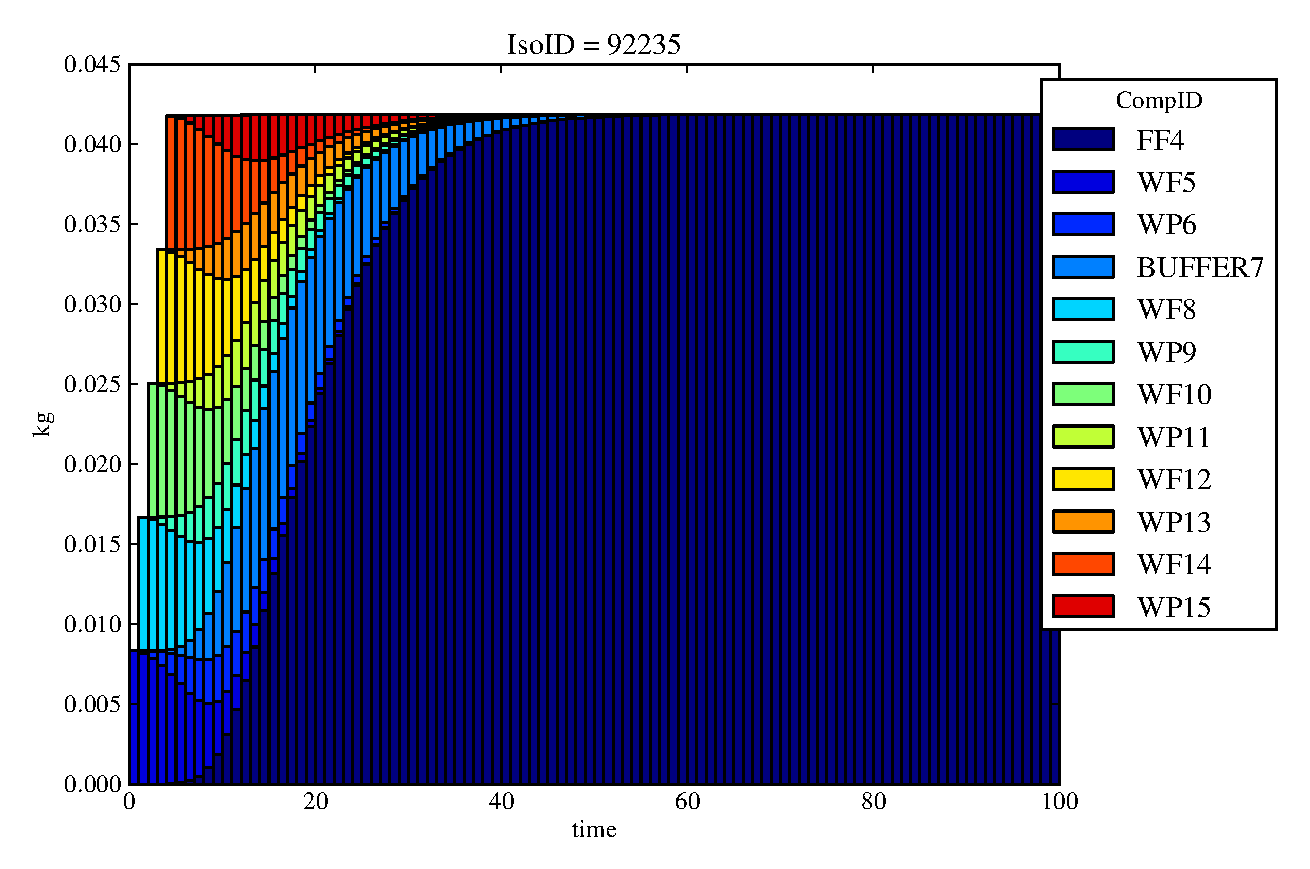
\includegraphics[width=0.6\textwidth]{./results/images/mcIII.eps}
\caption[$^{235}U$ residence. Mixed Cell Coupled Sorption and Solubility Limitation.]{
For the MCIII case in which containment is affected by solubility limitation,
        ($F_{d}=0.1$ for all components except far field), $^{235}U$ travels through waste 
        packages (WPN), their corresponding waste forms (WFN), and the surrounding 
        buffer (BUFFER7) more slowly than in the MCI case
        before permanent residence in the far field component (FF).
}
\label{fig:mcIIIall}
\end{figure}

\begin{figure}[ht]
\centering
  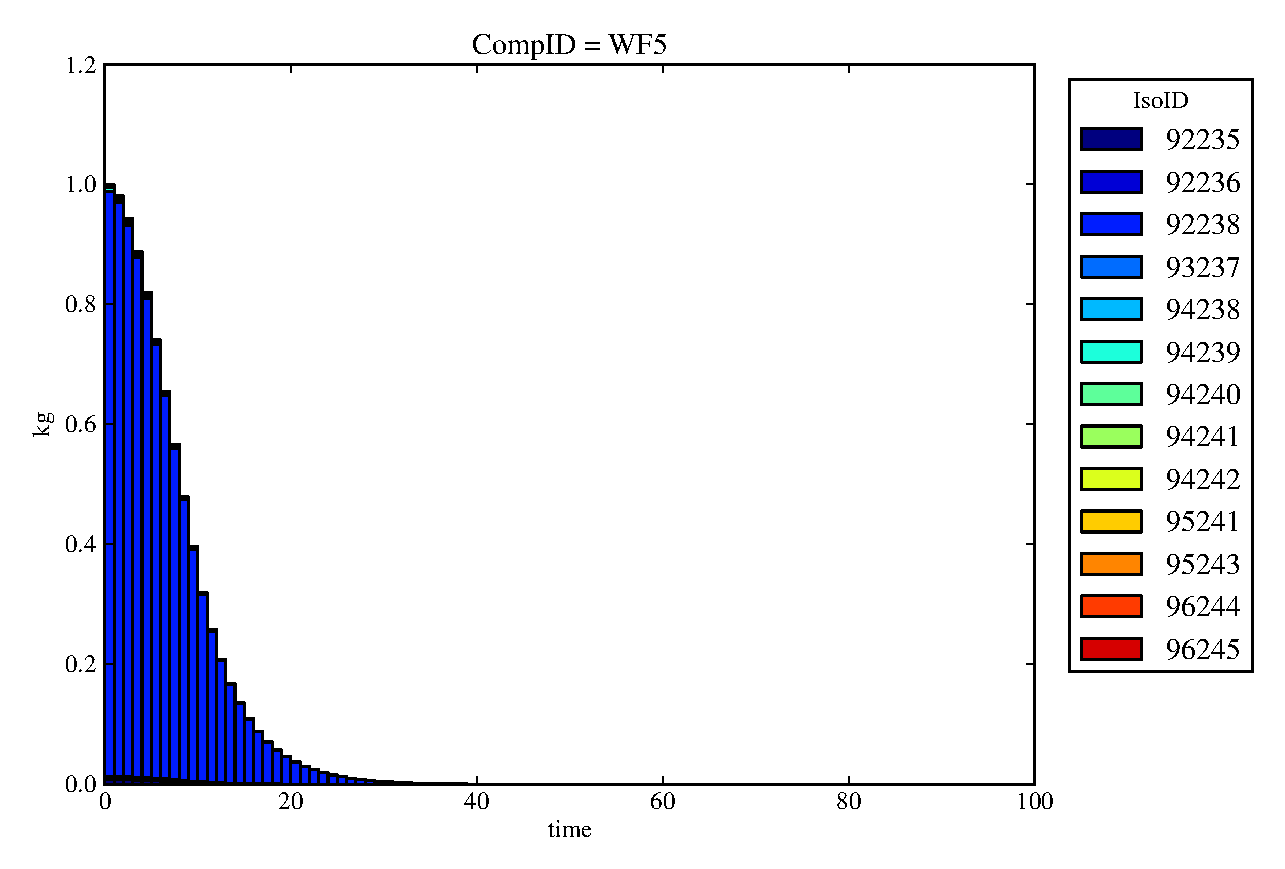
\includegraphics[width=0.6\textwidth]{./results/images/mcIII1.eps}
  \caption[Case MCIII Waste Form Contaminants.]{
          Waste Form 5 (degradation rate $F_d = 0.1[y^{-1}]$, reference solubility limit $S_{ref} = 0.001kg/m^3$) releases material with degradation.
    }
  \label{fig:mcIIIwf5}
\end{figure}


\begin{figure}[ht]
\centering
  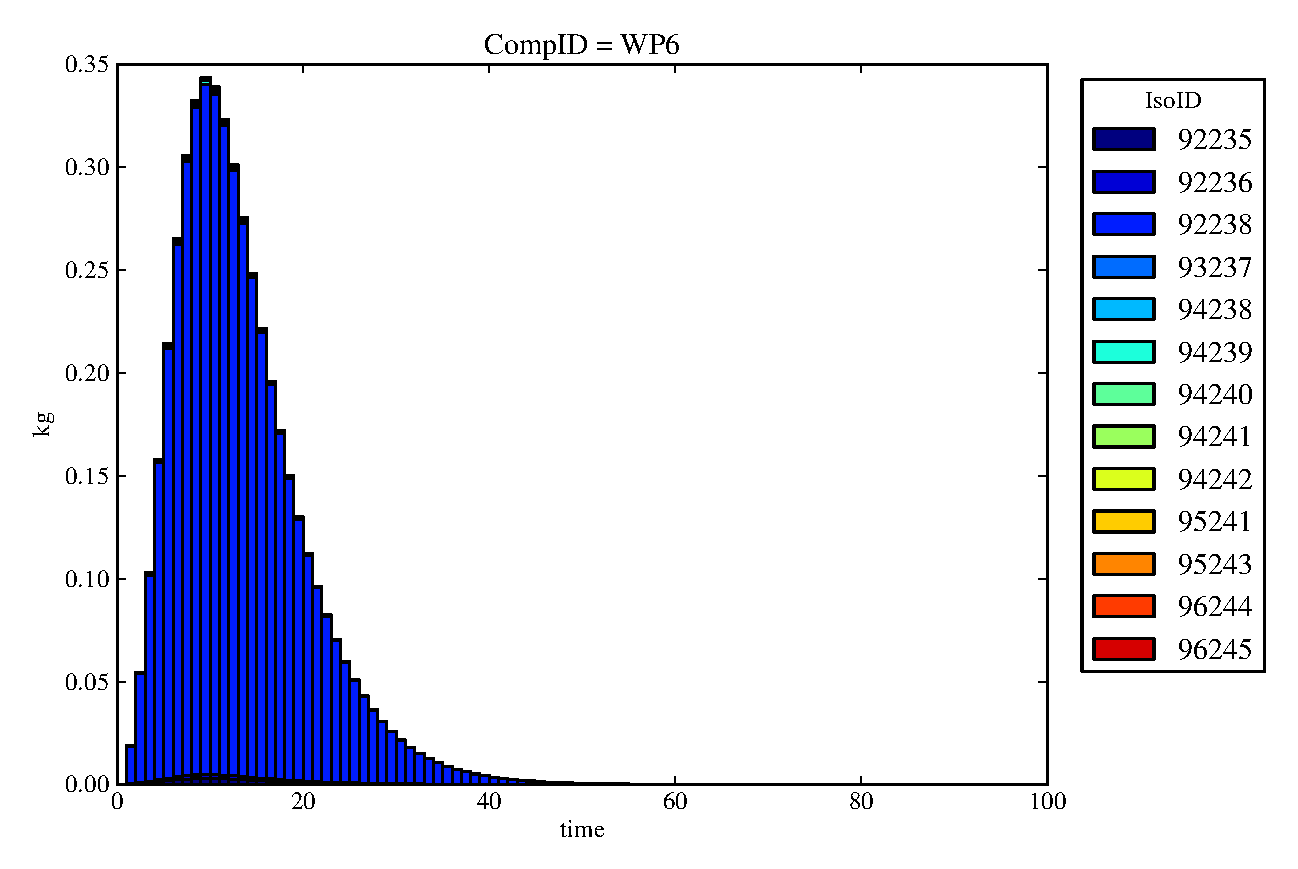
\includegraphics[width=0.6\textwidth]{./results/images/mcIII2.eps}
  \caption[Case MCIII Waste Package Contaminants.]{
          Waste Package 6 (degradation rate $F_d = 0.1[y^{-1}]$, reference solubility limit $S_{ref}=0.001kg/m^3$) receives then releases material.
    }
  \label{fig:mcIIIwp6}
\end{figure}

\begin{figure}[ht]
\centering
  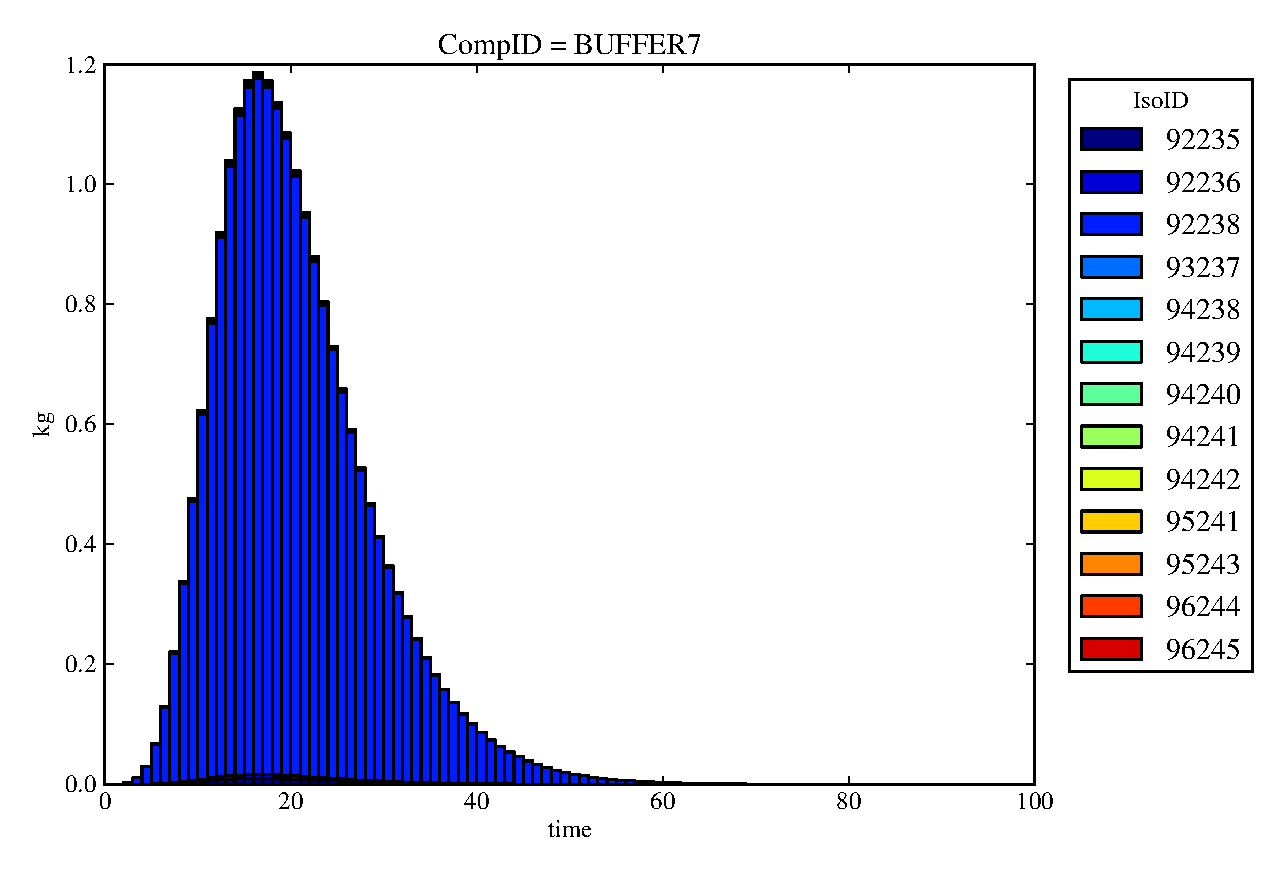
\includegraphics[width=0.6\textwidth]{./results/images/mcIII3.eps}
  \caption[Case MCIII Buffer Contaminants]{
          The Buffer, component 7 (degradation rate $F_d=0.1[y^{-1}]$, reference solubility 
        limit $S_{ref}=0.001kg/m^3$), receives and then releases material.
    }
  \label{fig:mcIIIbuff}
\end{figure}

\begin{figure}[ht]
\centering
  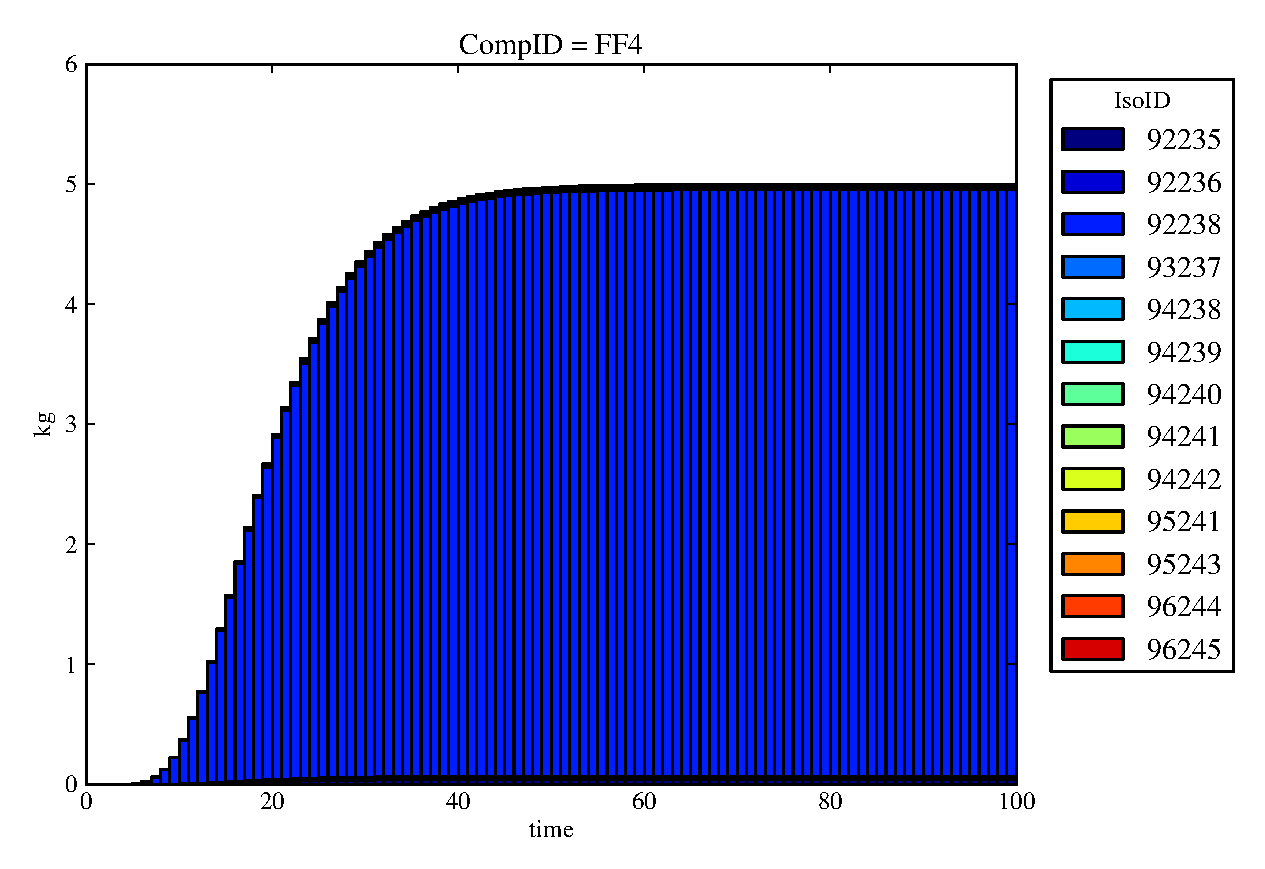
\includegraphics[width=0.6\textwidth]{./results/images/mcIII0.eps}
  \caption[Case MCIII Far Field Contaminants.]{All material is released into
        the Far Field, component 4 (degradation rate $F_d=0.0[y^{-1}]$, reference solubility limit $S_{ref} = 0.001kg/m^3$).}
  \label{fig:mcIII}
\end{figure}



\FloatBarrier



\subsection{Single Effect Parametric Analyses}
% Many parametric analysis were conducted to validate system responses

Each of the radionuclide contaminant transport models described in Section
\ref{sec:nuclide_models} capture different combintations of physics present in
the hydrologic contaminant transport problem. To determine how effectively
these physics were captured, single-effect simulations were conducted with
\Cyder and compared to similar analysis \cite{huff_key_2012} conducted with a
more detailed radionuclide transport model, the Clay \gls{GDSM}
\cite{clayton_generic_2011}. The Clay \gls{GDSM} was developed by the \gls{UFD}
Campaign within the \gls{DOE} Office of Nuclear Energy using the GoldSim
simulation environment \cite{golder_associates_goldsim_2010}. Hydrologic
contaminant transport in the Clay \gls{GDSM} relies on the GoldSim contaminant
transport module \cite{golder_associates_goldsim_2010-1}.

These single-effect sensitivity analyses were constructed by repeated
multi-component simulation runs conducted across the valid range for a single
parameter. To verify the behavior of a single parameter of each of the \Cyder
models, one hundred multi-component simulations were conducted, each with a
different value of that parameter.  This parametric analysis was conducted to
show that, for an arbitrary isotope, the expected dependence on that parameter
is captured. In the case of real isotopes in a full simulation, the same model
will be invoked with real parameters for each isotope. Thus, the this model
agreement is representative in all cases.

The results acheived with \Cyder were compared to the results of a similiar
parametric sensitivity analysis using the Clay \gls{GDSM} which was reported in
\cite{huff_key_2012}.

\subsubsection{Solubility Sensitivity}
Each of the radionuclide contaminant transport models described in Section
\ref{sec:nuclide_models} capture different combintations of physics present in
the hydrologic contaminant transport problem. To determine how effectively
these physics were captured, single-effect simulations were conducted with
\Cyder and compared to analysis was conducted with a more detailed radionuclide
transport model, the Clay \gls{GDSM} \cite{clayton_generic_2011}. The Clay
\gls{GDSM} was developed by the \gls{UFD} Campaign within the \gls{DOE} Office
of Nuclear Energy and relies on the GoldSim simulation environment
\cite{golder_associates_goldsim_2010} and its contaminant transport module
\cite{golder_associates_goldsim_2010-1}.

These single-effect sensitivity analyses were constructed by repeated
multi-component simulation runs conducted accross the valid range for a single
parameter.

To verify the behavior of the solubility limitation model in the Mixed Cell
model, for example, one hundred multi-component simulations were conducted,
each with a different reference solubility limit. This parametric analysis was
conducted to show that, for an arbitrary isotope, the expected solubility
limitation behavior is captured. In the case of real isotopes in a full
simulation, the same model will be invoked with real parameters for each
isotope. Thus, the this model agreement is representative in all cases.

The results acheived with \Cyder were compared to the results of a parametric
sensitivity analysis using the Clay \gls{GDSM} reported in
\cite{huff_key_2012}. That analysis showed that for solubility limits below a
certain threshold, the dose releases were directly proportional to the
solubility limit, indicating that the radionuclide concentration saturated the
groundwater up to the solubility limit near the waste form.  For solubility
limits above the threshold, however, further increase to the limit had no
effect on the peak dose. This demonstrates the situation in which the
solubility limit is so high that even complete dissolution of the waste
inventory into the pore water is insufficient to reach the solubility limit.

\begin{figure}[ht]
\begin{center}
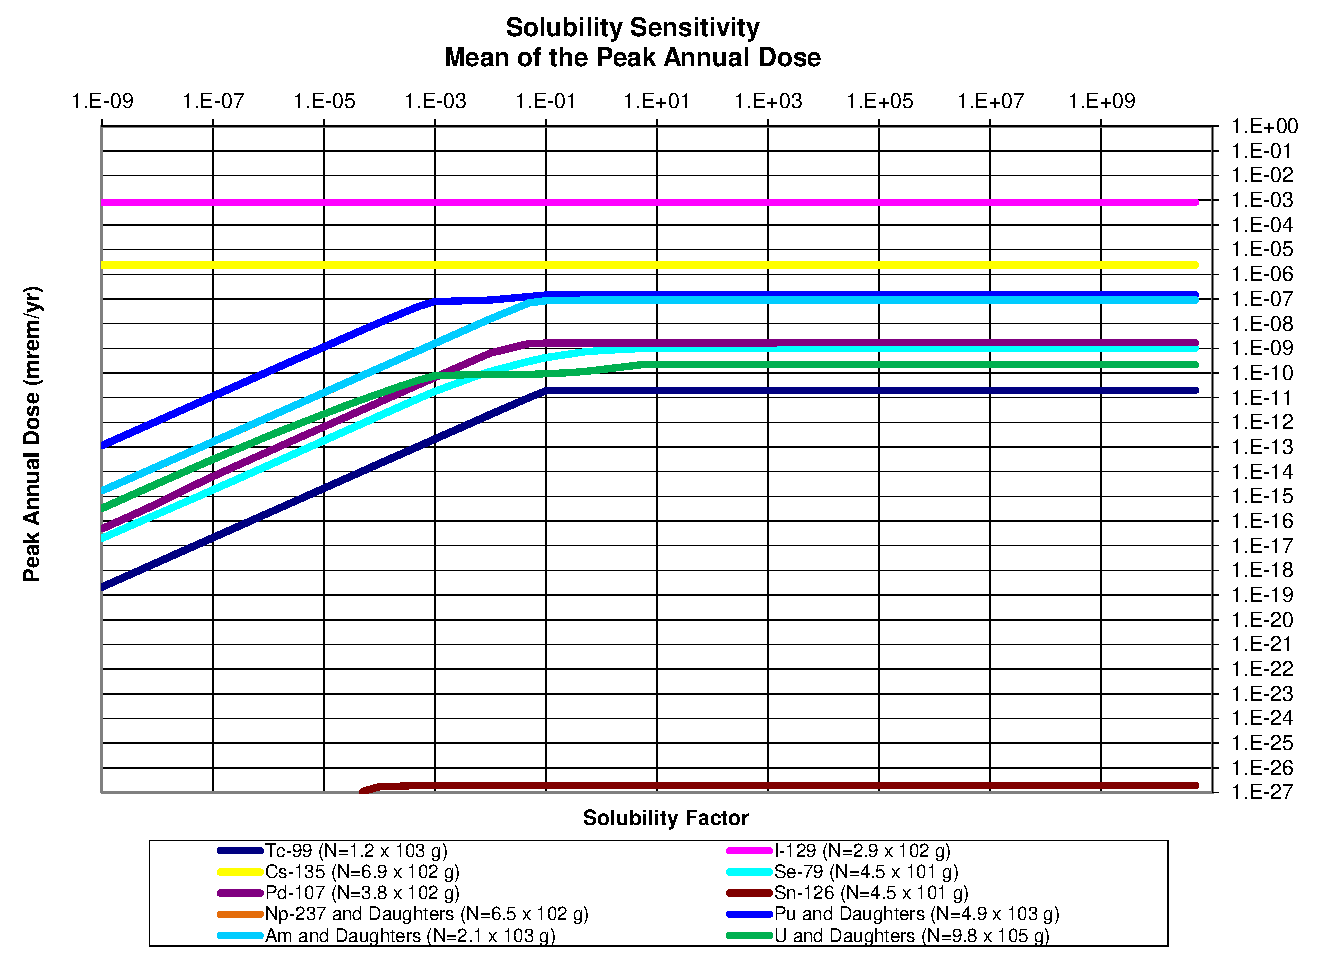
\includegraphics[width=0.7\linewidth]{./results/images/Solubility_Summary_SolFactor.eps}
\caption[Solubility factor sensitivity in GDSM Clay model]{Solubility factor sensitivity. The peak annual dose due to an inventory, $N$, of each isotope. This result was acheived with a parametric analysis using a detailed model of a generic clay repository \ref{huff_key_2012}}
\label{fig:SolSumFactor}
\end{center}
\end{figure}

\begin{figure}[ht]
\begin{center}
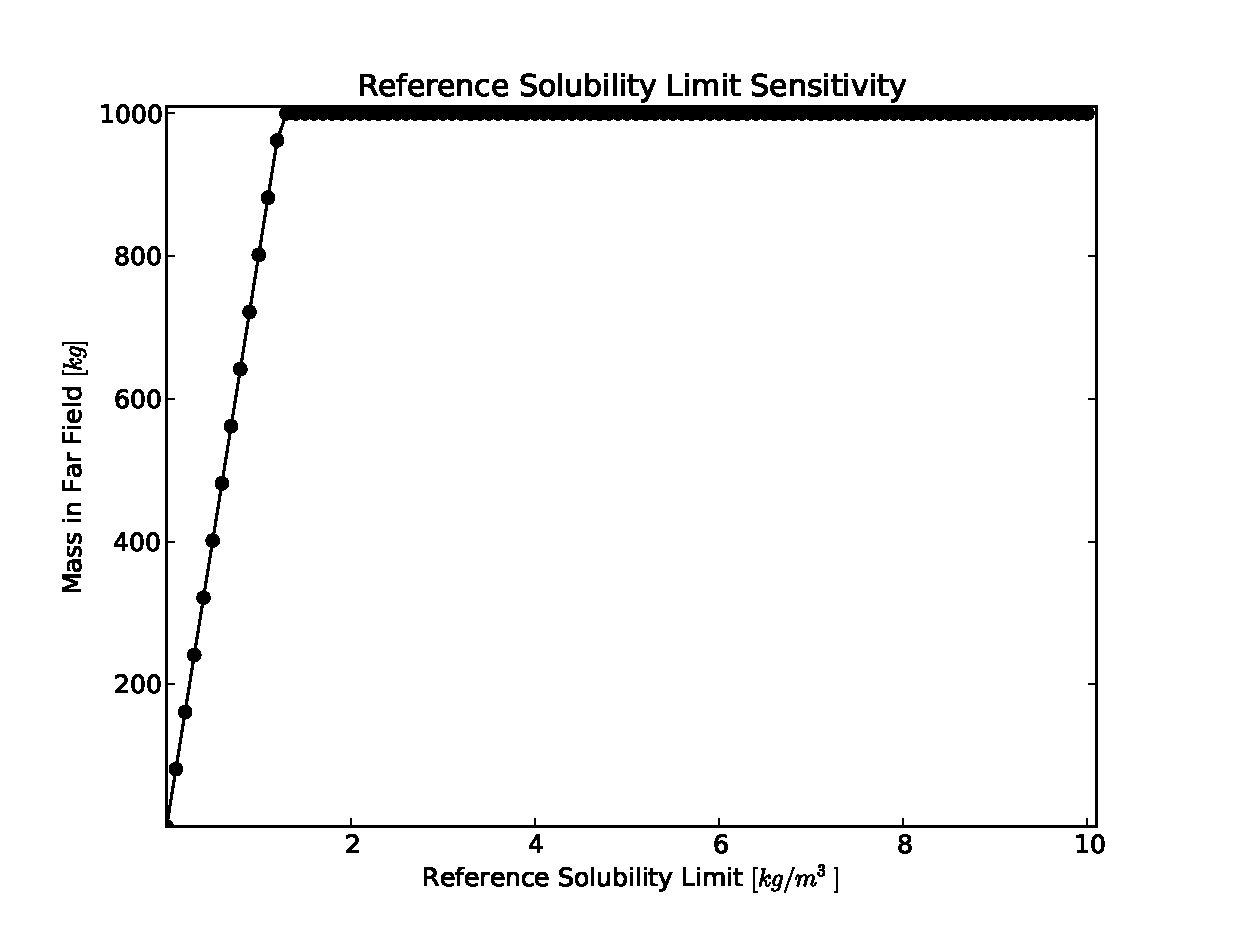
\includegraphics[width=0.7\linewidth]{./results/images/sol.eps}
\caption[Solubility Sensitivity in the Mixed Cell Model]{Sensitivity demonstration of solubility limitation in \Cyder for an arbitrary isotope assigned a variable solubility limit.}
\label{fig:sol_result}
\end{center}
\end{figure}


The results in Figure \ref{fig:SolSumFactor}, from the detailed parametric
analysis in \cite{huff_key_2012}, it is clear that for
solubility constants lower than the saturation threshold, the transport regime is solubility
limited and the relationship between peak annual dose and solubility limit is
strong.  Above the threshold, the transport regime is inventory limited
instead.

In the corresponding parametric analysis of \Cyder performance, it was shown that the
solubility sensitivity behavior closely matched that of the \gls{GDSM}
sensitivity behaviors. Specifically, in Figure \ref{fig:sol_result}, a sharp turnover
is seen where the solubility limit exceeds the point at which it limits
movement. For increased solubility limits, release remains constant, as
expected.

%\begin{figure}[ht]
%\begin{center}
%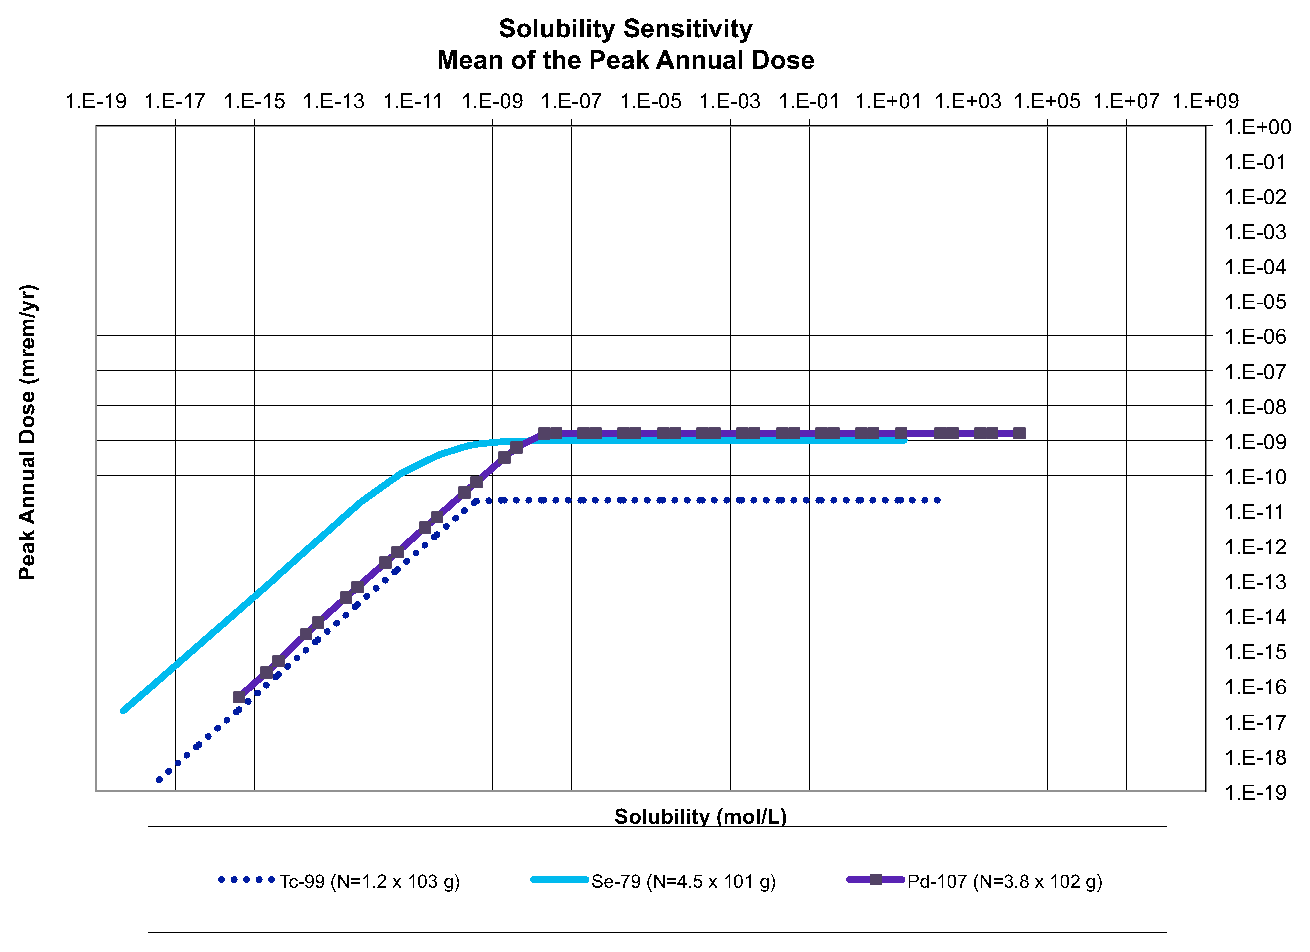
\includegraphics[width=0.7\linewidth]{./results/images/Solubility_Summary_Sol.eps}
%\caption[Solubility limit sensitivity in GDSM Clay model]{Solubility limit sensitivity. The peak annual dose due to an inventory,
%$N$, of each isotope.}
%\label{fig:SolSum}
%\end{center}
%\end{figure}


\FloatBarrier
\subsubsection{Sorption Sensitivity}

\input{./results/kd_sensitivity}
\input{./results/kd_results}

\FloatBarrier
\subsubsection{Waste Form Degradation Rate Sensitivity}
\input{./results/wf_deg_inv_sensitivity}
\input{./results/wf_deg_inv_results}

\FloatBarrier


\subsection{Significance}
% The existence of this code enables dynamic analysis of repository performance
% during fuel cycle simulation.

This work has provided a flexible software library for rapid medium-fidelity
calculation of generic repository performance in the context of fuel cycle
analysis.  Capable of hydrologic contaminant transport and integration within a
fuel cycle simulation library, \Cyder is the first of its kind.

In this work, modeling methods for geologic radioactive waste disposal
performance analysis were described as was their implementation in the \Cyder
repository performance library. The application programming interface to this
software library is intentionally general, facilitating the incorporation of
the models presented here within external software tools.

\Cyder performance within the \Cyclus fuel cycle simulator and agreement
between Cyder and a more detailed stand-alone model were also demonstrated.
\Cyder methods make a strategic tradeoff between speed and fidelity, capturing
essential physics when computing back-end nuclear fuel cycle metrics. The
result is a library of medium-fidelity hydrologic contaminant transport models
within a disposal facility simulation framework appropriate for use in dynamic
nuclear fuel cycle simulators.

The \Cyder source code is freely available to interested researchers and
potential model developers \cite{huff_cyder_2013}.  In addition to the source
code and supporting publications, the \Cyder library is well commented and
produces clickable, browsable automated documentation with each build. That
documentation is also available online.

Finally, this work contributes to an expanding ecosystem of computational
models available for use with the \Cyclus fuel cycle simulator. This hydrologic
nuclide transport library, by virtue of its capability to modularly integrate
with the \Cyclus fuel cycle simulator has laid the foundation for integrated
disposal option analysis in the context of fuel cycle options.


  \section{Acknowledgements}
This work was supported by the U.S.  Department of Energy, Basic Energy
Sciences, Office of Nuclear Energy, under contract \# DE-AC02-06CH11357.  This
work was also supported by the Department of Energy National Nuclear Security
Administration under Award Number DE‐NA0000979. Additionally, the author would
like to acknowledge the support of advisors Professor Paul P.H. Wilson and Dr.
W. Mark Nutt. All were instrumental in arriving at 
modeling decisions for this software.

  % References with bibTeX database:

  \bibliographystyle{elsarticle-num}
  \bibliography{bibliography}

  % Authors are advised to submit their bibtex database files. They are
  % requested to list a bibtex style file in the manuscript if they do
  % not want to use elsarticle-num.bst.

  \end{document}

  %
  % End of file `elsarticle-template-num.tex'.


